\chapter{Design of algorithm}\label{chap:algorithm}

The following table depicts the main correspondences relevant to our research:
\begin{equation}
\begin{tabular}{|c|c|c|}
\hline
\textbf{LOGIC} & \textbf{facts} & \textbf{rules} \\
& \mbox{human(socrates)} & $\forall x. \mbox{human}(x) \rightarrow \mbox{mortal}(x)$ \\
\hline
\textbf{ALGEBRA} & \textbf{element} & \textbf{element} \\
& $p \in \mathbb{A} $ & $(p \rightarrow q) \in \mathbb{A} $ \\
\hline
\textbf{WORLD} & \textbf{states} & \textbf{state transitions} \\
& $x_t$ & $x_t \stackrel{\squareF}{\mapsto} x_{t+1}$ \\
\hline
\end{tabular}
\end{equation}
The relation between LOGIC and WORLD has been elucidated quite thoroughly in the AI literature.  Note that the state $x_t$ is made up of a set of facts (logic propositions).  A single step of logic inference results in a new conclusion $\delta x$ which is \textit{added} (as a set element) to the current state $x_t$ to form a new state $x_{t+1}$.  Here $t$ refers to ``mental time'' which does not necessarily coincide with real time.

\section{From abstract algebraic logic to concrete computations}

There are two main routes to make abstract algebraic logic concrete:
\begin{itemize}
	\item Find \textbf{matrix representations} of the logical algebra
	\item Implement the logical algebra as the commutative algebra of (classical) \textbf{polynomials}
\end{itemize}

\section{What does it mean to train the AI?}

From the previous section,
\begin{equation}
F(x) = 0 \quad \mbox{is the solution to} \quad \dot{x} = f(x)
\end{equation}
and the two descriptions (by $F$ or by $f$) are equivalent.

The discrete version of $f$ is $\squaref$:
\begin{equation}
	\squaref(x_t) = x_{t+1} - x_t = \delta x
\end{equation}

The sensory data from the AI are a set of ``world'' points $\{ x_i \}$  and we require either:
\begin{equation}
F(x_t) = 0 \quad \mbox{or} \quad \squaref(x_t) = \delta x = x_{t+1} - x_t
\end{equation}
and $F$ or $f$ can be trained by gradient descent to eliminate errors in the above conditions (equations).

\begin{itemize}
	\item the $x_t$'s are represented as \textbf{logic facts}
	\item $F$ or $f$ is represented as \textbf{logic rules}
\end{itemize}
and we need to \textbf{evaluate} $F(x_t)$ or $f(x_t)$.

Let's do some examples:
% \usetagform{hidden}
\begin{equation}
\begin{tabular}{|c|c|}
\hline
\textbf{Logic formula} & \textbf{Algebraic form} \\
\hline
human(socrates) & h(s) = 1 \\
\hline
human(socrates) $\wedge$ human(plato) & h(s) $\cdot$ h(p) = 1 \\
\hline
human(socrates) $\rightarrow$ mortal(socrates) &  1 + h(s) + h(s) $\cdot$ m(s) = 1 \\
\hline
$\forall x.$ human($x$) & $h(x)$ is a propositional function \\
& $\forall_x h(x)$ is a constant function mapping to 1 or 0 \\
\hline
$\forall x.$ human($x$) $\rightarrow$ mortal($x$) & $\forall_x \bigl( 1 + h(x) + h(x) \cdot m(x) \bigr) $ \\
& is a constant function mapping to 1 or 0 \\
\hline
$\forall x,y,z.$ father($x,y$) $\wedge$ father($y,z$) $\rightarrow$ & $\forall_x \forall_y \forall_z \bigl( 1 + f(x,y) \cdot f(y,z) + f(x,y) \cdot f(y,z) \cdot g(x,z) \bigr) $ \\
grandfather($x,z$) & $\mapsto$ 0 or 1 \\
\hline
\textbf{general Horn formula}: & $\forall_{x...} \big( 1 + P \cdot Q \cdot R .... + P \cdot Q \cdot R ... \cdot Z \big) $ \\
$\forall_{x...} P \wedge Q \wedge R ... \rightarrow Z$ & $\mapsto$ 0 or 1 \\
\hline
\end{tabular}
\label{table:formulas}
\end{equation}

Now imagine there are millions of such rules.  Number of predicates obviously increases.

Does each equation require new variables, or can variables be re-used? Seems yes, can be re-used.

The \textbf{loss function} would be the sum of squared errors over all equations:
\begin{equation}
\mathcal{L} = \sum_{\mathrm{eqns}} \epsilon^2 = \sum_i \big( \phi_i (x...) - 1 \big)^2 .
\label{loss-function}
\end{equation}
Learning means to perform the \textbf{gradient descent} via $ \nabla_\Phi \mathcal{L} = \frac{\partial \mathcal{L}}{\partial \Phi} $ where $\Phi$ is the set of parameters for the equations.

Potential problems:
\begin{itemize}
	\item How to represent the set of equations efficiently?  Matrix of coefficients seems wasteful.
	\item We have lost the ``\textbf{deepness}'' of deep learning, but there is recent research showing that \textbf{shallow learning} may work well too.
	\item Need to iterate logical inference multiple times using the same set of equations.
\end{itemize}

How are new conclusions added to the state?  What is the state?  State = set of facts = set of \textbf{grounded} equations.

Inference:  how to get from current state to next state?  Big problem!!  New ground facts have to be read off from satisfaction of all equations.  Rather intractable...

See Chapter \ref{chap:background1}.

How to enumerate conclusions?  The loss function (\ref{loss-function}) can be trained on any data with correlations.  But what we have is data in the form of time series.  Need extra measures to ensure that equations only model $x_t \rightarrow x_{t+\Delta t}$.  Now how to enumerate conclusions?  From current state, iterate over all equations to generate new states.  This is getting very close to the classical logic-based AI inference algorithm.

The \textbf{interestingness function} gives a probability distribution over conclusions given the current ``context'' (which we identify as the current state $x_t$): $ \mathrm{Intg}(\delta x) = \mathbb{P}(\delta x | x_t) $.  This function has to be learned.  It has an equivariant structure due to the state as a set of propositions with permutation invariance.

One more efficiency problem:  iterating through all equations is inefficient, which brings back the necessity of the classical \textbf{rete algorithm}:  instead of matching rules against the state, we should match the current state against rules.  In other words, instead of $\delta x := \bigcup_i \mathrm{rule}_i (x)$, perform $\delta x := \text{compiled-rules}(\Delta x) $, where $\Delta x$ is the change of the current state from the previous state, and $\delta x$ is the change from the current state to the next state.

But we may also avoid the rete algorithm by stacking logical equations into \textbf{layers}, thus getting an efficiency advantage similar to deep learning.  A ``single'' step of logic inference would mean going through multiple layers of logic rules (equations).  

\section{``Geometric'' logic inference algorithm}

\begin{equation}
\vcenter{\hbox{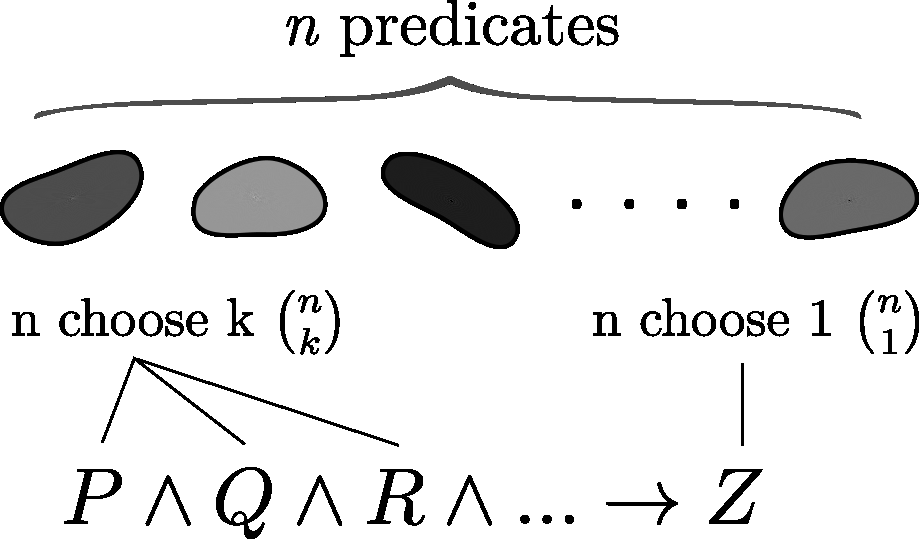
\includegraphics[scale=0.5]{geometric-logic-algorithm.png}}}
\end{equation}

\begin{itemize}
	\item What is a logic fact within a state?
	\item How does a rule generate a single new fact?
\end{itemize}

A fact consists of a point (in subject space) and a predicate that contains it.  The point itself does not suffice because it can belong to various predicates.  

To apply a rule, each \textbf{atomic term} in the rule has to be satisfied.  For each predicate $Q()$, this is verified by testing if we have any points among the facts contained in $Q$.

If we have \textsf{father(john, pete)} as a fact then we certainly can satisfy \textsf{father}$(x,y)$.  But we already have the point \textsf{(john, pete)} which may satisfy other predicates $Q(x,y)$.  So our method is slightly more permissive (and thus more powerful) in rules matching.

How does the rule's RHS generate a new fact?  It should also be a (point, predicate) pair.  The point has to \textbf{match} the premise.  How could this be ensured?

Secondly, the output predicate may not cover the point.

The matching process:  syntactically, we look at each literal in the rule and see if any fact unifies with the literal.  Geometrically, it means taking a point and checking if it lies inside a predicate.  If the fact is a (point, predicate) pair then it is given that the point belongs to the predicate, so it is not necessary to check for membership.  The result is simply taking the point when the predicates match.  But we still need to keep track of which variables the point coordinates are binding to.

The matching of the second literal will also return a point, but its coordinates would be bound to different dimensions.  

The binding of coordinates would be the basis of verifying the rule LHS.

RHS:  The bound variables (in various dimensions) need to be projected to the output space.  It may or may not be covered by the output predicate.  If not, the rule does \textit{not} apply.  This is in accord with the principle that rules should not change during inference.

\section{Computer representation of rules}

Each logic rule may vary in the following ways:
\begin{itemize}
	\item number of literals and their polarity
	\item number of arguments
	\item each argument may be a logic variable or logic constant
	\item which specific logic variable or constant.
\end{itemize}
\#1 and \#2 can be fixed.

For \#3 and \#4, each variable or constant may be represented by a pair $(p, \gamma)$ where $p$ is a point in the Subject Space, and $\gamma$ is the \textbf{cylindrification factor} representing the degree to which this argument is like a point or like a ``for all'' variable.  But this is problematic as the dimension of the Subject Space $X$ is not the same as the dimension of the variable space $\{ v_1, v_2, ... , v_n \}$.

In fact, each argument is $n$ copies of the Subject Space, ie, $X^n$.  One or more of the copies may be \textbf{cylindrified}.

There are two senses of the word ``cylindrify.''  Think for example the change from (John, Mary) to ($x$, Mary) as in ``everyone loves Mary.''  In the first sense, the point John on the $x$-coordinate becomes ``everyone,'' ie, the entire $x$-dimension becomes a cylinder.  In the second sense, a cylinder appears on the $y$-axis at the position of Mary:
\begin{equation}
\vcenter{\hbox{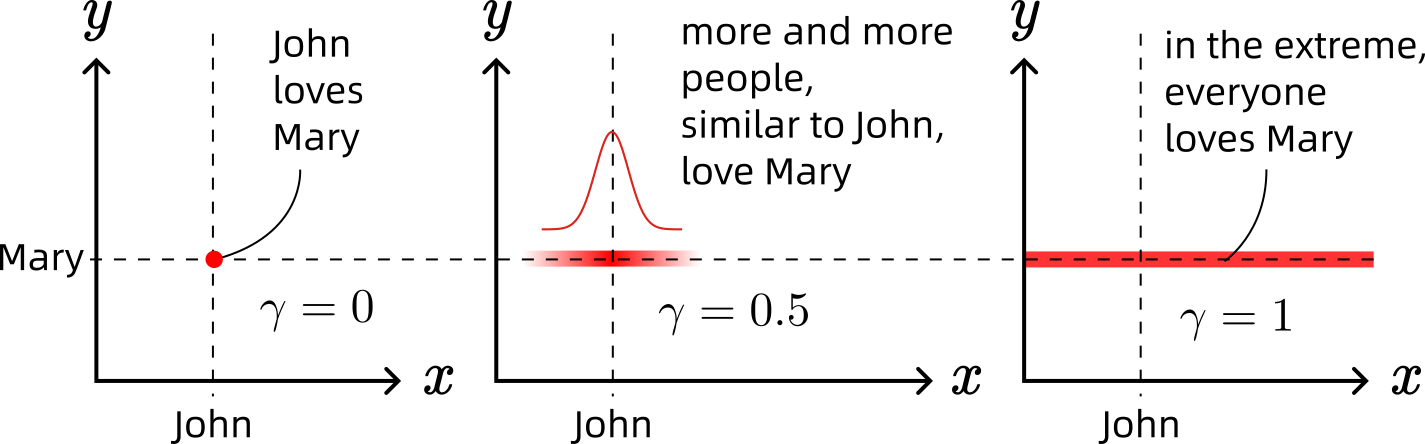
\includegraphics[scale=0.7]{cylindrify-example.png}}}
\end{equation}
In the above example, we have two copies of the Subject Space $X$, each is 1-dimensional.

The dimension $n$ is not just the number of variables appearing in one predicate in a rule, but the total number of variables appearing in a rule.

We suggest the following values (for a general human-level intelligent agent):
\begin{equation}
\begin{tabular}{|c|c|c|}
	\hline
	\textbf{Variable} & \textbf{Symbol} & \textbf{Suggested values} \\
	\hline
	\# of rules & $M$ &  millions up \\
	\hline
	\# of literals per rule & $K$ &  2-10, typical 3,4 \\
	\hline
	\# of arguments per rule & $n$ & 2, 3, 4  \\
	\hline
	Subject Space dimension & dim $X$ &  100-1000, typical 512, 768 \\
	\hline
\end{tabular}
\end{equation}

Is everything differentiable?

\section{Rules recommender}

The rules recommender would be a set function:
\begin{equation}
\mathsf{Ru}: \{ \mbox{current state} \} \rightarrow \{ \mbox{set of rules} \}
\end{equation}
which has equivariant structure on both its input and output.  This suggests the \textbf{Transformer} architecture is suitable for learning this function.

But this is clearly \textbf{non-differentiable}!  

In binary logic a rule either applies or does not apply.  To make the entire set of rules differentiable, rule application must be ``graded''.

So we propose a \textbf{probabilistic} rule-matching mechanism:
\begin{equation}
\vcenter{\hbox{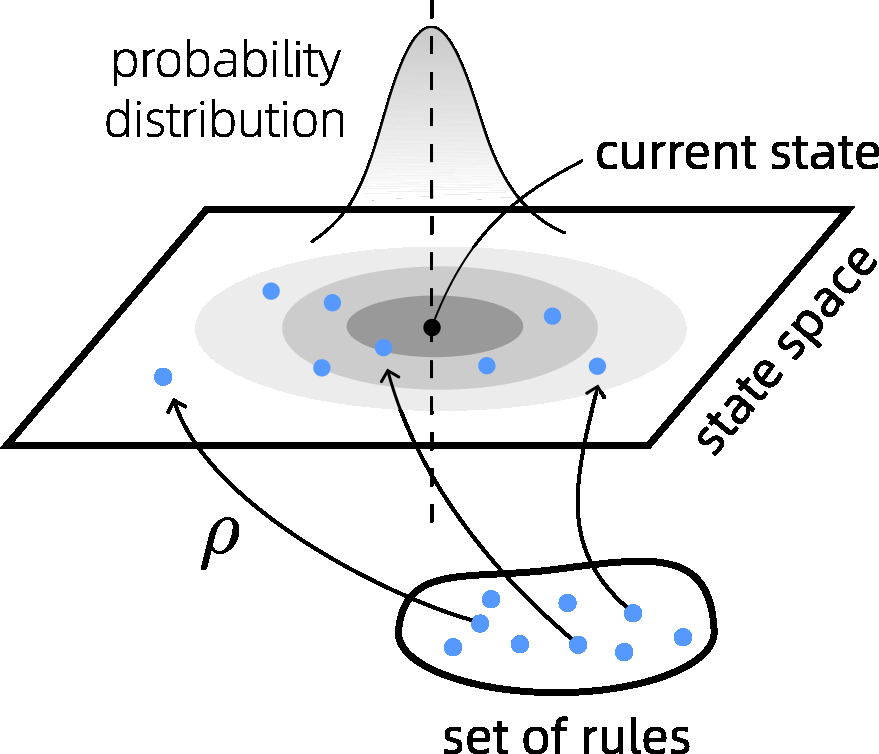
\includegraphics[scale=0.7]{rules-recommender.png}}}
\end{equation}
Rules are mapped by a function $\rho$ to the state space, such that rules are located close to the states they are most likely to match (this is a multi-objective optimization problem).  Given a current state $x$, denote the ball around it as $B(x, d)$.  The rules we predict most likely to match $x$ are given by $\rho^{-1}(B(x,d))$ for some distance $d$.  We can assign a Gaussian probability distribution centered around $x$ over such rules, so that rules are selected \textbf{probabilistically} for update.

It seems that doing so would not affect the convergence (of the learning algorithm) of the rules, but it would be much more efficient as the probability distribution is \textit{more} concentrated around $x$, so that large numbers of rules need \textit{not} be evaluated (for each state, at each time step).

% Rule 產生了新的結論,但先前選擇的 rule 是否影響新的 context?
% 其實 rules 本身可以分層。 最高的 rules 選擇下層的某些 rules。  但這只是其中一種做法。
% 其實如果有某 decision tree 負責 rules 的分流,似乎也仍然是可微的?
% but if the leafs of the decision tree are SHARED, differentiability may be a problem?
% the sorting tree can be deterministic... how does that affect differentiability?
% perhaps the rules at a whole can be regarded as a single function transforming the current state to the next state.  Differentiability would be discussed with respect to this function.
% What does it mean for differentiability to be broken...?  The total rule function must change infinitesimally per each update... 
% differentiation is like dy/dx.... when x = the total function...  the question is whether we can always perform x+dx... where dx will not be of finite length
% the state x will change from step to step....  but that's not a problem...  we care about the 

\begin{equation}
x_{t+1} = \squareF(x_t; \Theta)
\end{equation}
where $\Theta$ are all the parameters that determine the rules, $\squareF$ is the total function aggregating all the rules.  If we vary any one rule parameter, does it change abruptly?  The parameters $\Theta$ include the rules-sorting function $\rho$.

For gradient descent we need to calculate $\nabla_\Theta \mathcal{L}$ where $\Theta$ are all the parameters of rules, and the loss function is defined as the sum of errors over all rules, $\displaystyle \mathcal{L} = \sum_{\text{all rules}} \epsilon^2 $.  Each error usually is given by the difference as compared against a reference value (supervised learning), but in our case such a value is unavailable, instead the objective comes from reinforcement learning, ie, the Hamilton-Jacobi-Bellman equation:  $J(x_{t+1}) = \max_a [ \gamma J(x_t) + R(x_t,a) ] $, where $a$ means \textbf{action}.  In the logic-based setting, an action means applying a logic rule to change the state.  

Policy function:
\begin{equation}
\pi: X \times A \rightarrow [0,1]
\end{equation}
By the \textbf{Policy Gradient Theorem}, calculation of $\nabla_\Theta J$ translates to calculating $\nabla_\Theta \pi$.

\section{Interestingness}

This can be implemented implicitly by making the inference algorithm output a probability distribution over all deduced conclusions and then picking the most probable one.
